\section*{\nr.4 \titfour (25 Punkte)}
\begin{enumerate}[(a)]
\item Ist das Teilchen perfekt in einem Kasten eingeschlossen, so müssen an den Rändern die Knoten der Wellenfunktion liegen. Die Wellenfunktion selbst beschreibt eine stationäre stehende Welle, das heißt, ihr Betragsquadrat ist nicht nicht zeitabhängig, da ein gebundener Zustand vorliegt.
\item In der Vorlesung wurde gezeigt, dass sich die stehenden Wellen im Kastenpotential in der Form
\begin{equation}
\psi_n(x,t) = 2i A \sin(k_n x) e^{i\omega_n t}
\end{equation}
schreiben lassen, mit einer geeigneten Normierung $A \in \mathbb{C}$, wobei $|A|=1/\sqrt{2d}$. Zur Erfüllung der Randbedingungen muss
\begin{equation}
k_n d = (n+1) \pi; \quad n\in \mathbb{N}_{\geq 0} 
\end{equation}
erfüllt sein, wobei $n$ die Anzahl der Knoten ohne Rand bezeichnet. Mit $k_n = 2\pi/\lambda_n$ folgt direkt für die Wellenlänge:
\begin{equation}
\lambda_n = \frac{2d}{n+1}
\end{equation}
und für den Impuls $p_n = h/\lambda$:
\begin{equation}
p_n = \frac{(n+1)\pi}{2d}
\end{equation}
Die Funktion der Aufenthaltswahrscheinlichkeitsdichte ist durch
\begin{equation}
|\psi_n(x)|^2 = \frac{2}{d} \sin^2\left[{\frac{(n+1)\pi x}{d}}\right]
\end{equation}
gegeben. Skizzen finden sich in \vref{fig:aufenthalt}.
\begin{figure}[htbp]
\centering
% GNUPLOT: LaTeX picture with Postscript
\begingroup
  \makeatletter
  \providecommand\color[2][]{%
    \GenericError{(gnuplot) \space\space\space\@spaces}{%
      Package color not loaded in conjunction with
      terminal option `colourtext'%
    }{See the gnuplot documentation for explanation.%
    }{Either use 'blacktext' in gnuplot or load the package
      color.sty in LaTeX.}%
    \renewcommand\color[2][]{}%
  }%
  \providecommand\includegraphics[2][]{%
    \GenericError{(gnuplot) \space\space\space\@spaces}{%
      Package graphicx or graphics not loaded%
    }{See the gnuplot documentation for explanation.%
    }{The gnuplot epslatex terminal needs graphicx.sty or graphics.sty.}%
    \renewcommand\includegraphics[2][]{}%
  }%
  \providecommand\rotatebox[2]{#2}%
  \@ifundefined{ifGPcolor}{%
    \newif\ifGPcolor
    \GPcolortrue
  }{}%
  \@ifundefined{ifGPblacktext}{%
    \newif\ifGPblacktext
    \GPblacktextfalse
  }{}%
  % define a \g@addto@macro without @ in the name:
  \let\gplgaddtomacro\g@addto@macro
  % define empty templates for all commands taking text:
  \gdef\gplbacktext{}%
  \gdef\gplfronttext{}%
  \makeatother
  \ifGPblacktext
    % no textcolor at all
    \def\colorrgb#1{}%
    \def\colorgray#1{}%
  \else
    % gray or color?
    \ifGPcolor
      \def\colorrgb#1{\color[rgb]{#1}}%
      \def\colorgray#1{\color[gray]{#1}}%
      \expandafter\def\csname LTw\endcsname{\color{white}}%
      \expandafter\def\csname LTb\endcsname{\color{black}}%
      \expandafter\def\csname LTa\endcsname{\color{black}}%
      \expandafter\def\csname LT0\endcsname{\color[rgb]{1,0,0}}%
      \expandafter\def\csname LT1\endcsname{\color[rgb]{0,1,0}}%
      \expandafter\def\csname LT2\endcsname{\color[rgb]{0,0,1}}%
      \expandafter\def\csname LT3\endcsname{\color[rgb]{1,0,1}}%
      \expandafter\def\csname LT4\endcsname{\color[rgb]{0,1,1}}%
      \expandafter\def\csname LT5\endcsname{\color[rgb]{1,1,0}}%
      \expandafter\def\csname LT6\endcsname{\color[rgb]{0,0,0}}%
      \expandafter\def\csname LT7\endcsname{\color[rgb]{1,0.3,0}}%
      \expandafter\def\csname LT8\endcsname{\color[rgb]{0.5,0.5,0.5}}%
    \else
      % gray
      \def\colorrgb#1{\color{black}}%
      \def\colorgray#1{\color[gray]{#1}}%
      \expandafter\def\csname LTw\endcsname{\color{white}}%
      \expandafter\def\csname LTb\endcsname{\color{black}}%
      \expandafter\def\csname LTa\endcsname{\color{black}}%
      \expandafter\def\csname LT0\endcsname{\color{black}}%
      \expandafter\def\csname LT1\endcsname{\color{black}}%
      \expandafter\def\csname LT2\endcsname{\color{black}}%
      \expandafter\def\csname LT3\endcsname{\color{black}}%
      \expandafter\def\csname LT4\endcsname{\color{black}}%
      \expandafter\def\csname LT5\endcsname{\color{black}}%
      \expandafter\def\csname LT6\endcsname{\color{black}}%
      \expandafter\def\csname LT7\endcsname{\color{black}}%
      \expandafter\def\csname LT8\endcsname{\color{black}}%
    \fi
  \fi
    \setlength{\unitlength}{0.0500bp}%
    \ifx\gptboxheight\undefined%
      \newlength{\gptboxheight}%
      \newlength{\gptboxwidth}%
      \newsavebox{\gptboxtext}%
    \fi%
    \setlength{\fboxrule}{0.5pt}%
    \setlength{\fboxsep}{1pt}%
\begin{picture}(7936.00,5102.00)%
    \gplgaddtomacro\gplbacktext{%
      \csname LTb\endcsname%
      \put(814,1048){\makebox(0,0)[r]{\strut{}$0$}}%
      \put(814,1909){\makebox(0,0)[r]{\strut{}$0.5$}}%
      \put(814,2770){\makebox(0,0)[r]{\strut{}$1$}}%
      \put(814,3632){\makebox(0,0)[r]{\strut{}$1.5$}}%
      \put(814,4493){\makebox(0,0)[r]{\strut{}$2$}}%
      \put(2411,484){\makebox(0,0){\strut{}$0$}}%
      \put(4243,484){\makebox(0,0){\strut{}$0.5$}}%
      \put(6074,484){\makebox(0,0){\strut{}$1$}}%
    }%
    \gplgaddtomacro\gplfronttext{%
      \csname LTb\endcsname%
      \put(176,2770){\rotatebox{-270}{\makebox(0,0){\strut{}$|\psi_{n}(x)|^2$}}}%
      \put(4242,154){\makebox(0,0){\strut{}$x$}}%
      \csname LTb\endcsname%
      \put(6552,4664){\makebox(0,0)[r]{\strut{}$n = 0$}}%
      \csname LTb\endcsname%
      \put(6552,4444){\makebox(0,0)[r]{\strut{}$n = 1$}}%
    }%
    \gplgaddtomacro\gplbacktext{%
      \csname LTb\endcsname%
      \put(814,1048){\makebox(0,0)[r]{\strut{}$0$}}%
      \put(814,1909){\makebox(0,0)[r]{\strut{}$0.5$}}%
      \put(814,2770){\makebox(0,0)[r]{\strut{}$1$}}%
      \put(814,3632){\makebox(0,0)[r]{\strut{}$1.5$}}%
      \put(814,4493){\makebox(0,0)[r]{\strut{}$2$}}%
      \put(2411,484){\makebox(0,0){\strut{}$0$}}%
      \put(4243,484){\makebox(0,0){\strut{}$0.5$}}%
      \put(6074,484){\makebox(0,0){\strut{}$1$}}%
    }%
    \gplgaddtomacro\gplfronttext{%
      \csname LTb\endcsname%
      \put(176,2770){\rotatebox{-270}{\makebox(0,0){\strut{}$|\psi_{n}(x)|^2$}}}%
      \put(4242,154){\makebox(0,0){\strut{}$x$}}%
      \csname LTb\endcsname%
      \put(6552,4664){\makebox(0,0)[r]{\strut{}$n = 0$}}%
      \csname LTb\endcsname%
      \put(6552,4444){\makebox(0,0)[r]{\strut{}$n = 1$}}%
    }%
    \gplbacktext
    \put(0,0){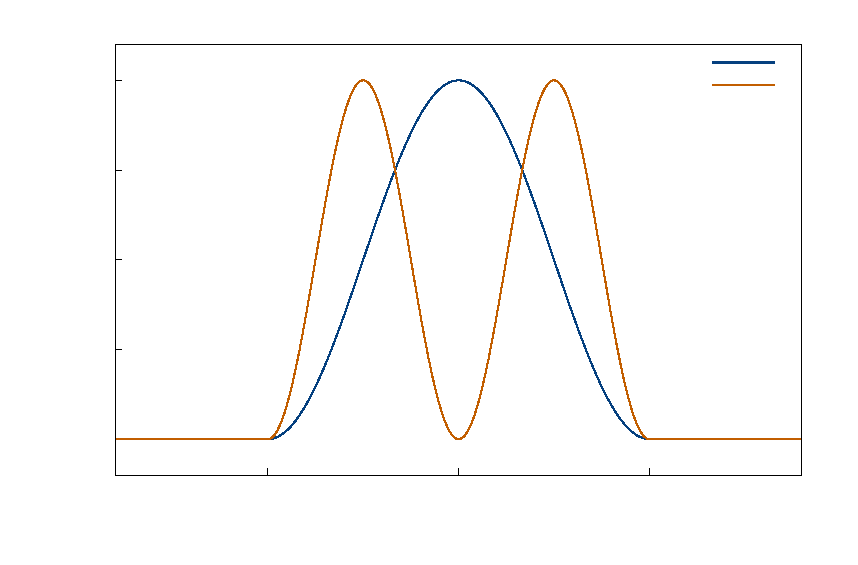
\includegraphics{aufenthalt}}%
    \gplfronttext
  \end{picture}%
\endgroup

\caption{$|\psi_n(x)|^2$ für $d=1$ in \emph{einheitenlosen} Größen.}
\label{fig:aufenthalt}
\end{figure}

\item Für die kinetische Energie $E_n$ folgt mit $E_n=p_n^2/(2m)$:
\begin{equation}
E_n = \frac{(n+1)^2\pi^2}{8d^2m}
\end{equation}
Insbesondere folgt für $n=0$:
\begin{equation}
E_0 = \frac{\pi^2}{8d^2m}
\end{equation}

Im Grenzübergang $d \to\infty$ muss, damit die Energie endlich und nichtverschwindend bleibt, die Knotenzahl über alle Grenzen wachsen. Bei graphischer Abbildung ist ab einer hinreichend großen Knotenzahl die Diskretisierung nicht mehr erkennbar und im Grenzübergang wird die Funktion kontinuierlich.

\item Sowohl für Photonen als auch für massive Teilchen gilt die Beziehung
\begin{equation}
p = \frac{h}{\lambda},
\end{equation}
wobei sie für letztere die die de-Broglie-Beziehung darstellt. Für die Energie eines Photons gilt weiter:
\begin{equation}
E = h\nu = \frac{hc}{\lambda}
\end{equation}
Aus der relativistischen Energie-Impuls-Beziehung
\begin{equation}
E = \sqrt{p^2c^2 + m^2 c^4} = \sqrt{\frac{h^2c^2}{\lambda^2} + m^2 c^4}
\end{equation}
sieht man jedoch, dass für massive Teilchen ($m\neq 0$) die Energie-Wellenbeziehung anders ist, was daher rührt, dass die (Gruppen-)Geschwindigkeit von massiven Teilchen unterhalb der Lichtgeschwindigkeit liegt, d.h. $\lambda_\text{massiv} \cdot \nu_\text{massiv} < c$.
\end{enumerate}